\chapter{Zbiory danych}

\section{Charakterystyka zbioru MNIST}
Pierwszym obiektem, na którym przeprowadzono badania jest popularny w uczeniu maszynowych zbiór danych MNIST (ang. \textit{Modified National Institute of Standards and Technology}). Składający się łącznie około 70 000 obrazów (60 000 przykładów testowych oraz około 10 000 przykładów treningowych), przedstawia ręcznie pisane cyfry od 0 do 9. Każdy z obrazów domyślnie posiada rozmiar 28x28 pikseli, co w efekcie daje 784 piksele (cechy) dla każdego rozważanego obrazu. Cały zbiór danych reprezentowany jest w skali szarości, co oznacza, że każdy piksel przyjmuje wartość z zakresu od 0 do 255, gdzie 0 oznacza kolor czarny, natomiast 255 kolor biały. Przykładowe obrazy z tego zbioru danych przedstawiono na rysunku \ref{fig:1_mnist_samples}.

\begin{figure}[htbp]
    \centering
    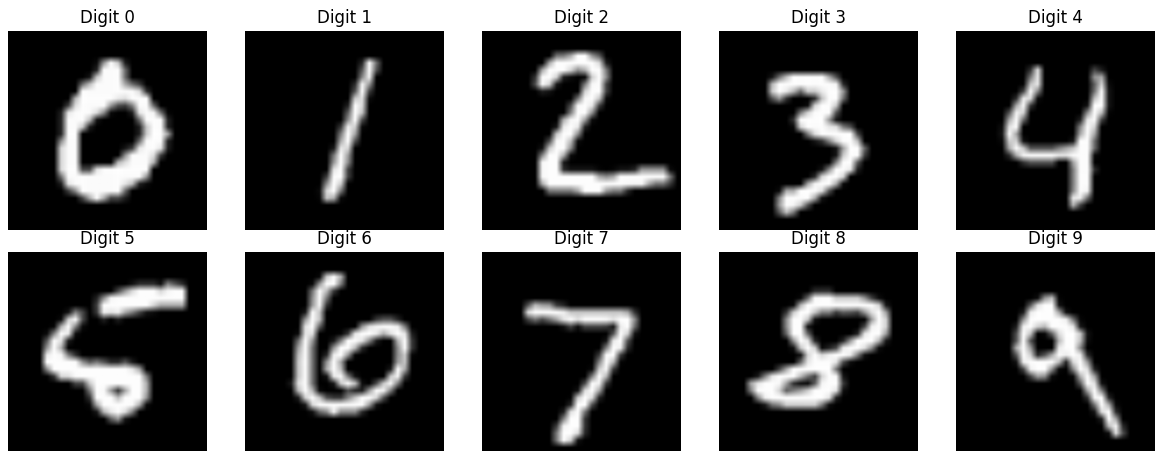
\includegraphics[width=0.7\textwidth]{imgs/1_mnist.png}
    \caption{Przykładowe obrazy z zbioru MNIST}
    \label{fig:1_mnist_samples}
\end{figure}

Cechą zbioru MNIST jest jego zbalansowany charakter, co oznacza, że każda z etykiet jest reprezentowana przez podobną ilość przykładów uczących w zbiorze. Zbalansowany zbiór danych jest kluczowy w zadaniach klasyfikacji, ponieważ pozwala na uniknięcie problemu tendencyjności modelu podczas późniejszej klasyfikacji nowych danych, których model wcześniej nie widział. Zdecydowano się na wykorzystanie opisywanego zbioru ze względu na jego popularność i prostotę. Skala szarości, która przekłada się na prostotę zbioru danych pozwala na wstępne zapoznanie się ze specyfiką wyników generowanych przez badane algorytmy wyjaśnialnej sztucznej inteligencji, co stanowi dobrą bazę do dalszych eksperymentów z bardziej złożonymi zbiorami danych.

\section{Charakterystyka zbioru CIFAR-10}

Kolejnym zbiorem danych, który wykorzystano w badaniach jest również popularny zbiór CIFAR-10 (ang. \textit{Canadian Institute for Advanced Research}). Zbiór ten charakteryzuje się podobną ilością przykładów, co omawiany wcześniej MNIST. Podobnie jak poprzednik, CIFAR-10 posiada 10 klas, jednak w w przeciwieństwie do MNIST, klasy te reprezentują różne obiekty, takie jak samochody, samoloty, ptaki etc. Od poprzednika różni się również rozmiarem obrazów. W tym przypadku mamy do czynienia z danymi o rozmiarze 32x32 pikseli, co daje 1024 cechy. Z racji, że CIFAR-10 jest zbiorem danych kolorowych, liczbę tę należy pomnożyć przez 3 (kanały RGB), co daje łącznie 3072 cechy dla każdego obrazu. Przykładowe obrazy z tego zbioru danych przedstawiono na rysunku \ref{fig:2_cifar_samples}.

\begin{figure}[htbp]
    \centering
    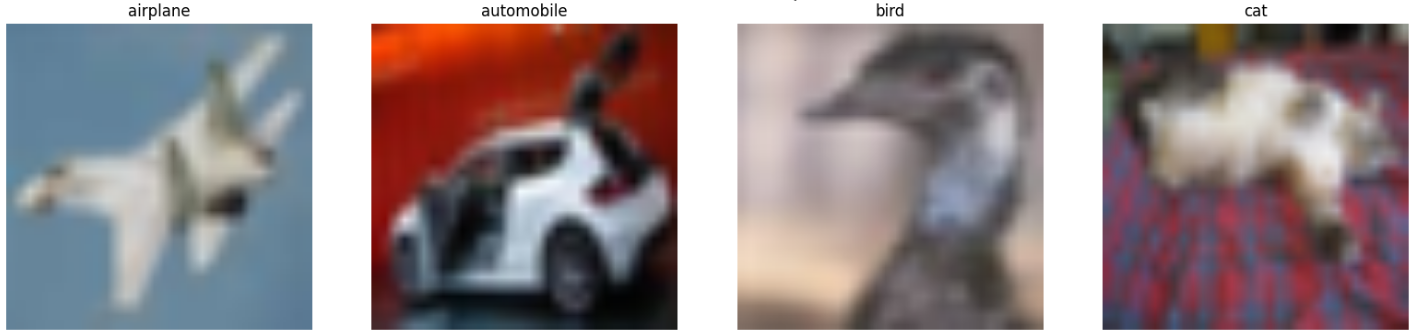
\includegraphics[width=0.7\textwidth]{imgs/2_cifar.png}
    \caption{Przykładowe obrazy z zbioru CIFAR-10}
    \label{fig:2_cifar_samples}
\end{figure}

Analogicznie jak w przypadku MNIST, CIFAR-10 jest zbiorem danych zbalansowanym, co oznacza, że każda z klas jest reprezentowana przez podobną ilość przykładów uczących. Wybór omawianego zbioru danych był podyktowany potrzebą zbadania algorytmów wyjaśnialnej sztucznej inteligencji w warunkach danych bardziej złożonych, które odzwierciedlają realistyczne scenariusze (różne gatunki zwierząt, obiekty, tło itp.). Ze względu na swoją różnorodność stanowi doskonały test dla badanych algorytmów, pozwalając na ocenę ich skuteczności w kontekście bardziej złożonych danych.
